\documentclass{beamer}

% Encoding and language support
\usepackage[T2A]{fontenc}
\usepackage[utf8]{inputenc}
\usepackage[russian]{babel}

% Packages for math and graphics
\usepackage{amsmath}
\usepackage{graphicx}
\usepackage{booktabs} % For better tables
\usepackage{ragged2e} % For text alignment

% Minimalist theme
\usetheme{default}

% Black-and-white color scheme
\setbeamercolor{background canvas}{bg=white}
\setbeamercolor{normal text}{fg=black}
\setbeamercolor{title}{fg=black}
\setbeamercolor{author}{fg=black}
\setbeamercolor{date}{fg=black}
\setbeamercolor{frametitle}{fg=black}
\setbeamercolor{itemize item}{fg=black}
\setbeamercolor{itemize subitem}{fg=black}
\setbeamercolor{enumerate item}{fg=black}

\setbeamertemplate{title page}{
	\vspace*{0.5cm}
	\begin{center}
		\includegraphics[height=1.1cm]{logo.jpg} % Логотип (можно удалить)
		\vskip0.5cm
		
		{\usebeamerfont{title}\bfseries\large\inserttitle\par}
		\vskip0.8cm
		
		{\usebeamerfont{author}\small
			\textbf{Кромачев М.А.}, гр. 5030102/10201\par}
		\vskip0.3cm
		
		{\usebeamerfont{institute}\footnotesize
			СПбПУ Петра Великого\par
			Физико-механический институт\par}
		\vskip0.8cm
		
		{\usebeamerfont{date}\footnotesize
			Научный руководитель: доц., к.ф.-м.н. И.Е. Ануфриев\par
			\insertdate\par}
	\end{center}
}

% Custom frame title without numbers
\setbeamertemplate{frametitle}{
	\vspace*{0.3cm}
	\begin{beamercolorbox}[wd=\textwidth]{frametitle}
		\usebeamerfont{frametitle}\insertframetitle
	\end{beamercolorbox}
	\vspace*{0.2cm}
}

% Add page number in bottom right corner (except title page)
\setbeamertemplate{footline}{
	\ifnum\insertframenumber=1\else% Skip title page
	\hfill\scriptsize\insertframenumber/\inserttotalframenumber\hspace*{0.5cm}\vspace{0.5cm}
	\fi%
}

% Itemize style
\setbeamertemplate{itemize item}{\color{black}$\bullet$}
\setbeamertemplate{itemize subitem}{\color{black}$\circ$}

% Text alignment
\setbeamertemplate{blocks}[rounded][shadow=false]
\justifying

% Remove navigation symbols
\setbeamertemplate{navigation symbols}{}

\title{Децентрализованное решение задачи о назначениях целей группе роботов}
\author{}
\date{\today}

\begin{document}
	
	\begin{frame}[plain]
		\titlepage
	\end{frame}

	\begin{frame}
		\frametitle{Содержание}
		\begin{itemize}
			\item Сущность задачи
			\item Классификация робототехнических систем
			\item Положения, выносимые на защиту
			\item Формальная постановка задачи
			\item Венгерский метод
			\item Алгоритм аукционного торга
			\item Описание аукционного алгоритма
			\item Модификация алгоритма аукционного торга
			\item Описание модифицированного аукционного алгоритма
			\item Результаты экспериментов
			\item Требования к  исследуемому алгоритму
		\end{itemize}
	\end{frame}
	
	\begin{frame}
	    \frametitle{Сущность задачи}
	    \begin{columns}[T]
	        \begin{column}{0.5\textwidth}
	            \begin{itemize}
	                \item Цели \raisebox{-0.3em}{\includegraphics[width=0.5cm]{3.png}}  
	                \item Роботы {\includegraphics[width=0.5cm]{2.jpg}}  
	                \begin{itemize}
	                    \item Радиус связи
	                    \item Область видимости
	                \end{itemize}
	                \item Центр управления \raisebox{-0.1em}{\includegraphics[width=0.5cm]{1.jpg}}  
	                \item Погрешность определения координат целей
	            \end{itemize}
	        \end{column}
	        \begin{column}{0.6\textwidth}
	            \centering
		 \hspace*{-1.5cm} % Отрицательный отступ для смещения влевоы
	            \includegraphics[width=\textwidth,height=0.85\textheight,keepaspectratio]{mrta1.png}
	        \end{column}
	    \end{columns}
	\end{frame}

	\begin{frame}
		\frametitle{Классификация робототехнических систем}
		\centering
		\includegraphics[width=\textwidth,height=0.95\textheight,keepaspectratio]{classification.png}
	\end{frame}


	\begin{frame}
		\frametitle{Положения, выносимые на защиту}
		\begin{itemize}
			\item \textbf{Принятые допущения:}
				\begin{itemize}
					\item Все роботы имеют одинаковый и неизменный радиус связи
					\item Все роботы обладают одинаковыми скоростями движения
					\item Каждый робот видит все цели
					\item Точность определения координат целей одинакова для всех роботов
					\item Не учитываются динамические системы роботов
				\end{itemize}
			\item \textbf{Постановка задачи}
			\item \textbf{Итерационный децентрализованный алгоритм назначения целей роботам:}
				\begin{itemize}
					\item Учет ограниченного радиуса связи (R)
					\item Управление точностью решения через параметр (\(\varepsilon\))
				\end{itemize}
			\item \textbf{Результаты исследований}
			\item \textbf{Требования к  исследуемому алгоритму}
		\end{itemize}
	\end{frame}

	\begin{frame}{Формальная постановка задачи}
		\vspace*{-0.2cm}
		\small
		\textbf{Дано:}
		\begin{itemize}
			\item Множество роботов $R = \{r_1, r_2, \ldots, r_n\}$.
			\item Множество целей $T = \{t_1, t_2, \ldots, t_m\}$.
			\item Матрица затрат $C = \{c_{ij}\}$, где $c_{ij}$ --- время, необходимое роботу $i$ для достижения цели $j$.
		\end{itemize}
		
		\textbf{Цель:} Минимизировать суммарные затраты
		\[
		\sum_{i=1}^n c_{i j_i} \rightarrow \min,
		\]
		где $j_i$ --- цель, назначенная роботу $r_i$.
		

		\vspace*{0.1cm}
		\textbf{Ограничения:}
		\begin{itemize}
			\item Каждый робот получает не более одной цели: $\sum_{j=1}^m x_{ij} \leq 1, \ \forall i = 1, \ldots, n$.
			\item Каждая цель назначается не более чем одному роботу: $\sum_{i=1}^n x_{ij} \leq 1, \ \forall j = 1, \ldots, m$.
			\item $x_{ij} \in \{0, 1\}$, где $x_{ij} = 1$, если робот $i$ назначен цели $j$, иначе $x_{ij} = 0$.
		\end{itemize}
	
	\end{frame}

	

	\begin{frame}
		\frametitle{Венгерский метод}
		\begin{columns}[T] % Параметр T выравнивает колонки по верху
			\begin{column}{0.5\textwidth} % Левая колонка (текст)
				\begin{itemize}
					 \item Реализация требует либо централизованного управления, либо параллельного выполнения алгоритма на всех роботах
                   				 \item Гарантирует точное оптимальное решение
                   				 \item Вычислительная сложность: $O(n^2 m)$
				\end{itemize}
			\end{column}
			\begin{column}{0.5\textwidth} % Правая колонка (изображение)
				\centering
				\includegraphics[width=\textwidth,height=0.85\textheight,keepaspectratio]{mrta2.jpeg}
			\end{column}
		\end{columns}
	\end{frame}
                

	\begin{frame}
	    \frametitle{Классический алгоритм аукционного торга}
	    \begin{columns}[T]
	        \begin{column}{0.6\textwidth}
	            \begin{itemize}
	                \item Нет единого центра управления
	                \item Имитирует процесс торгов
	                \item Параметр \(\varepsilon\) контролирует точность целевой функции
	                \item Требует полной связи между роботами
	                \item Число итераций до достижения точного решения $\sim m\cdot C/$\(\varepsilon\)
	            \end{itemize}
	        \end{column}
	        \begin{column}{0.4\textwidth}
	            \hspace*{-1cm} % Отрицательный отступ для смещения влево
	            \includegraphics[width=1.2\textwidth,height=0.85\textheight,keepaspectratio]{mrta3.jpeg}
	        \end{column}
	    \end{columns}
	\end{frame}

	
	\begin{frame}
		\frametitle{Описание классического аукционного алгоритма}
			\small	
			\begin{itemize}
				\item Матрица времен \( C \) преобразуется в матрицу выгод \( A \), где задача максимизации эквивалентна минимизации времени.
				\item \textbf{Инициализация}: 
				\begin{itemize}
					\item Установить цены целей: \( p_j = 0, \ \forall j \).
					\item Роботы не назначены на цели.
				\end{itemize}
				\item \textbf{«Почти счастье»}: 
				\[ \alpha_{i j_i} - p_{j_i} \geq \max_j \{\alpha_{ij} - p_j\} - \varepsilon.\]
				\item \textbf{Итерация для каждого робота} \( i \):
				\begin{itemize}
					\item Выбрать цель: \( j_i = \arg\max_j \{\alpha_{ij} - p_j\} \) (макс. выгода).
					\item Вычислить: 
					\begin{itemize}
						\item \( v_i = \max_j \{\alpha_{ij} - p_j\} \) (макс. выгода).
						\item \( w_i = \max_{j \neq j_i} \{\alpha_{ij} - p_j\} \) (вторая по величине выгода).
					\end{itemize}
					\item Переназначить робота \( i \) на цель \( j_i \).
					\item Обновить цену: \( p_{j_i} \gets p_{j_i} + (v_i - w_i + \varepsilon) \).
				\end{itemize}
				\item \textbf{Условие завершения}: Все роботы «почти счастливы».
			\end{itemize}
	\end{frame}


	\begin{frame}
		\frametitle{Модификация алгоритма аукционного торга}
		\begin{columns}[T] % Параметр T выравнивает колонки по верху
			\begin{column}{0.6\textwidth} % Левая колонка (текст)
				\begin{itemize}
					\item Нет единого центра управления
					\item Ограниченная связь между роботами (внутри связных компонент)
					\item Полная видимость целей для всех роботов
					\item Разделение роботов на связные компоненты по графу связи
					\item Независимый аукцион в каждой компоненте
				\end{itemize}
			\end{column}
			\begin{column}{0.4\textwidth} % Правая колонка (изображение)
				\centering
				\includegraphics[width=\textwidth,height=0.85\textheight,keepaspectratio]{mrta4.jpeg}
			\end{column}
		\end{columns}
	\end{frame}

	\begin{frame}
	    \frametitle{Описание модифицированного аукционного алгоритма}
	            \begin{itemize}
	                \item \textbf{А. Разбиение на компоненты:}
	                \begin{itemize}
	                    \item Робот $r_i$ определяет соседей: $v_{ik} = 1$, если $d(p_i, p_k) \leq R$, иначе $v_{ik} = 0$.
	                    \item Обмен идентификаторами с соседями ($v_{ik} = 1$) для определения компоненты $C_l$.
	                    \item Каждый робот знает свою $C_l$ и её состав.
	                \end{itemize}
	                \item \textbf{Б. Инициализация:}
	                \begin{itemize}
	                    \item Вычисление $c_{ij} = \frac{d(p_i, q_j)}{v_i}$ для целей $q_j$.
	                    \item Определение $C_{\max} = \max_{i \in C_l, j} c_{ij}$ в $C_l$.
	                    \item Выгоды: $\alpha_{ij} = C_{\max} - c_{ij}$; цены: $p_j = 0$; $j_i = -1$.
	                \end{itemize}
	                \item \textbf{В. Аукцион в $C_l$:}
	                \begin{itemize}
	                    \item Для $r_i \in C_l$: проверить $\alpha_{i j_i} - p_{j_i} \geq \max_j \{\alpha_{ij} - p_j\} - \varepsilon$.
	                    \item Если не почти счастлив: выбрать $j_i = \arg\max_j \{\alpha_{ij} - p_j\}$, вычислить $v_i$, $w_i$, обновить $p_{j_i} += v_i - w_i + \varepsilon$.
	                    \item Повторять до почти счастья всех роботов.
	                \end{itemize}
	            \end{itemize}
	\end{frame}
	
	\begin{frame}
	    \frametitle{Результаты экспериментов}
	    \small
	    \begin{columns}[T]
	        \begin{column}{0.5\textwidth} % Левая колонка (текст)
	            \hspace*{-0.5cm} % Смещение списка влево
	            \begin{itemize}
	                \item Точность аукционного алгоритма быстро растет на начальных итерациях, вплоть до значения относительной точности в 95\%.
	                \item Для больших n требуется больше итераций из-за увеличения числа конфликтов между роботами.
	            \end{itemize}
	        \end{column}
	        \begin{column}{0.65\textwidth} % Правая колонка (график)
	            \centering
	            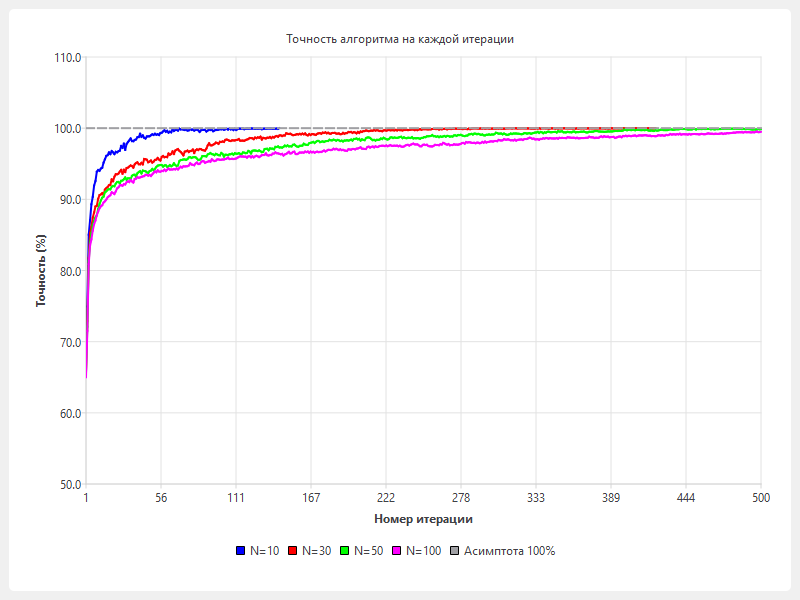
\includegraphics[width=\textwidth,height=0.7\textheight,keepaspectratio]{accuracy_per_iteration_chart.png}
	        \end{column}
	    \end{columns}
	\end{frame}
	
	\begin{frame}
	    \frametitle{Результаты экспериментов}
	    \small
	    \begin{columns}[T]
	        \begin{column}{0.5\textwidth} % Левая колонка (текст)
	            \hspace*{-0.5cm} % Смещение списка влево
	            \begin{itemize}
	                \item Аукционный алгоритм: меньше вычислительных операций, однако больше обменов
	                \item Эффективность зависит от $F_{\text{выч}}$ и $F_{\text{обм}}$
	                \item Аукцион лучше при высокой $F_{\text{обм}}$; венгерский — при высокой $F_{\text{выч}}$ 
	            \end{itemize}
	        \end{column}

	        \hspace*{-0.2cm}
	        \begin{column}{0.65\textwidth} % Правая колонка (график)
		      \vspace*{0.1cm}
	            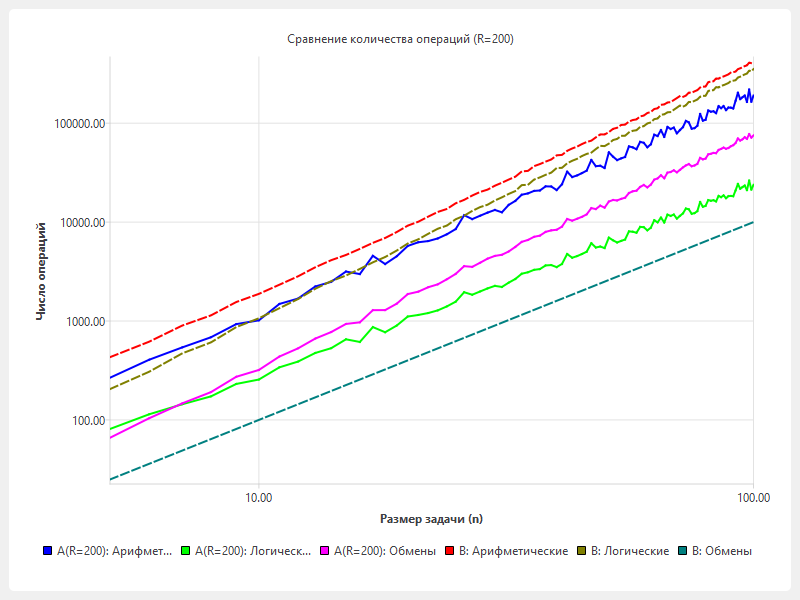
\includegraphics[width=\textwidth,height=0.7\textheight,keepaspectratio]{operation_chart.png}
	        \end{column}
	    \end{columns}
	\end{frame}
	
	\begin{frame}
	    \frametitle{Требования к  аукционному алгоритму}
	    \small
	    \begin{itemize}
	        \item Венгерский алгоритм, не учитывающий погрешности и лишённый параметра  $\varepsilon$, стремится к точному решению, которое в условиях реальных погрешностей и ограниченного радиуса связи недостижимо
	        \item Аукционный алгоритм, в отличие от венгерского, позволяет учитывать погрешности в измерениях матрицы выгод путём выбора параметра $\varepsilon$, что обеспечивает высокую точность при меньших вычислительных затратах
	        \item Алгоритм аукциона требует меньшего числа арифметических и логических операций по сравнению с венгерским, что делает его предпочтительным при высоких скоростях обмена данными, несмотря на большее число итераций
	    \end{itemize}
	\end{frame}
	
\end{document}